\documentclass[letterpaper,10pt,conference]{ieeeconf}
\IEEEoverridecommandlockouts
\overrideIEEEmargins
\usepackage[T1]{fontenc}
\usepackage{times}
\usepackage{amsmath,amssymb}
\usepackage{graphicx}
\usepackage{booktabs}
\usepackage{array}
\usepackage{url}
\renewcommand{\topfraction}{0.95}
\renewcommand{\textfraction}{0.05}
\newcommand{\V}{\mathrm{V}}
\newcommand{\C}{\mathrm{C}}
\newcommand{\U}{\mathrm{U}}
\title{BiSafeBench: Safety Evaluation of LLM-Generated\\Bimanual Programs and Their Safeguards}
\author{Anonymous authors}
\begin{document}
\maketitle
\thispagestyle{empty}
\pagestyle{empty}
\raggedbottom
\suppressfloats[t]

\begin{abstract}
Generated robot programs can fail before a safety-critical operation is ever reached. A low violation rate can therefore reflect missing behavior rather than correct execution. We introduce BiSafeBench, a benchmark for evaluating LLM-generated bimanual programs and their safeguards. It links the requested task graph, generated source, execution trace, and requirement-level evidence. This separates missing structure, unreached operations, and executed violations. Safeguards are scored against evidence for the same requirement. Across 384 natural programs spanning 16 task families, third-review adjudication identifies 248 as UNSAFE under the finite benchmark contract. Re-scoring unchanged safeguard outputs preserves four recurring blind spots: attribute composition, buffer ownership, long dependencies, and event protocols. Controlled studies locate composition failures at distinct stages. Concurrent generation reduces structural fidelity and deep-path exposure. In a separate coherent-authorization study, an explicit stable-pair interface reduces the concurrency-by-window interaction in slot-level failure by 67.19 percentage points. The tested capability profiles do not exhibit a monotone safety improvement. BiSafeBench diagnoses where program construction, execution, and protection diverge from task requirements.
\end{abstract}

\section{Introduction}
\begin{figure}[t]
\centering

\includegraphics[width=\columnwidth]{figures/figure1.png}
\caption{BiSafeBench study overview. Recorded handover frames provide physical task context; the 384-program natural corpus and controlled studies support distinct requirement-grounded analyses. The photographs and illustrative task-world renderings are not execution evidence for the generated programs. Figure~\ref{fig:design} follows one frozen program from source to requirement verdict.}
\label{fig:overview}
\end{figure}
Language models are becoming robot programmers. Systems such as Code as Policies and RoboScript translate high-level instructions into executable perception, planning, and control logic~\cite{cap,roboscript}. This interface is powerful because generated code can make state-dependent decisions. It is dangerous for the same reason: a robot can reach the requested final pose after violating ownership, synchronization, observation, or motion-lifecycle requirements along the way.

Consider a shared-buffer handover. Figure~\ref{fig:design} shows a generated program that completes its task despite entering the buffer before acquiring its lock. A different program may avoid this violation simply by omitting the requested concurrent behavior. A guard may instead stop execution without restoring the task. These outcomes call for different remedies. A safety score must distinguish them.

Safety evaluation already extends beyond task completion. Embodied benchmarks separate feasibility from danger, and SafeManip grounds reusable temporal properties in manipulation rollouts~\cite{safeagent,despite,safemanip}. Verification and runtime protection further constrain plans before or during execution~\cite{verifyllm,roboguard}. The remaining question for generated code is more specific: did the program construct the behavior that was supposed to be evaluated, and did its safeguard assess the right requirement?

BiSafeBench makes this question explicit by aligning the \emph{composition requested by the task}, the \emph{behavior implemented and reached by the program}, and the \emph{requirement assessed by each safeguard}. A task grammar defines the requested composition; structural checks and instrumented traces establish implementation and path exposure. Human review supplies requirement evidence independently of the safeguards under test. This alignment distinguishes missing behavior, executed violations, and failed protection at the same requirement.

Natural generation and controlled studies serve different purposes (Fig.~\ref{fig:overview}). The natural corpus exposes defects across every evaluated task family and recurring safeguard blind spots despite strong detection elsewhere. Controlled studies locate composition effects in program construction and coherent authorization. The structure-preserving supplement finds no further direct-risk increase under its tested transformations. Capability comparisons likewise do not support a monotone safety improvement across the tested profiles.

Our contributions are:
\begin{itemize}
\item \textbf{A program-to-evidence benchmark.} An executable task grammar and independent requirement evidence connect generated bimanual programs to the safeguards evaluated on them.
\item We characterize the natural defect spectrum across 16 task families and identify four recurring safeguard blind spots. Original dual review and third-review adjudication make their sensitivity to labels explicit.
\item Controlled comparisons locate composition failures upstream in program construction and in a specific coherent-authorization mechanism. The stable-pair interface sharply reduces the latter's failure interaction; capability comparisons show why a model rank cannot replace requirement-level evaluation.
\end{itemize}

\section{Related Work}
\subsection{From language plans to executable robot programs}
Language-based planning makes instructions actionable through admissible action sequences, grounded skills, and classical planning~\cite{zeroshotplanner,saycan,llmp}. Code as Policies, ProgPrompt, ChatGPT for Robotics, and RoboScript move this interface toward executable programs and robot APIs~\cite{cap,progprompt,chatgptrobotics,roboscript}.

Feedback and grounding further improve this interface. Inner Monologue, LLM-Planner, SayPlan, and VoxPoser incorporate observations, scene structure, or geometric representations~\cite{innermonologue,llmplanner,sayplan,voxposer}. AutoTAMP checks translated task-and-motion specifications, while CoPAL corrects planning and execution through feedback~\cite{autotamp,copal}. PaLM-E and RT-2 integrate perception, language, and action in embodied models~\cite{palme,rt2}. These systems enable and correct robot behavior. BiSafeBench asks whether generated control flow preserves the ownership, event, observation, and motion-lifecycle requirements of the requested task.

\subsection{Embodied, planning, and bimanual benchmarks}
ALFRED, ALFWorld, and BEHAVIOR-1K evaluate grounded household tasks and long-horizon behavior~\cite{alfred,alfworld,behavior1k}. PlanBench and ActionReasoningBench isolate planning, executability, state tracking, and action effects in symbolic domains~\cite{planbench,actionreasoning}. These benchmarks expose planning limits, but do not treat generated bimanual source code and its resource/event traces as the joint evaluation object.

Coordination adds requirements beyond individual task completion~\cite{dualarmsurvey}. RoCoBench makes parallel versus sequential decomposition, observation asymmetry, and workspace overlap explicit~\cite{roco}. ALOHA and PerAct2 study fine-grained or language-conditioned bimanual control~\cite{aloha,peract2}. BiManiBench evaluates spatial reasoning, action planning, and end-effector control; DuoBench uses stage-based semantic evaluation in simulation and hardware~\cite{bimanibench,duobench}. BiSafeBench complements these policy- and capability-centered evaluations by checking whether generated source implements and reaches the specified coordination structure.

\subsection{Safety benchmarks for embodied agents}
Safety benchmarks already distinguish task achievement from risk. SafeAgentBench evaluates hazardous instructions, Safe-BeAl couples task planning with safety alignment, and DESPITE measures feasibility and danger avoidance separately~\cite{safeagent,safebeal,despite}. BeSafe-Bench spans web, mobile, and embodied-agent environments~\cite{besafebench}; RoboPAIR studies attacks that induce harmful robot actions~\cite{robopair}.

SafeManip is a close execution-level counterpart. It maps manipulation rollouts to symbolic traces and checks reusable LTL$_f$ properties, reporting per-property violations separately from task success~\cite{safemanip}. Its protocol is policy-agnostic; the reported evaluation uses VLA policies. It also discusses limited progress and inactive monitors. Its unsafe-state exposure metric measures time spent unsafe; our path-exposure measure records whether a requirement's deciding operation was reached.

BiSafeBench changes the evaluation unit to generated source together with its requested task graph and reached behavior. The increment is not temporal monitoring alone. This alignment distinguishes omitted program structure from executed violations and scores safeguards against evidence for the same requirement.

\subsection{Formal planning, verification, and runtime protection}
Task-and-motion planning connects symbolic actions, geometric constraints, and execution~\cite{hiertamp,tampsurvey}. Language interfaces compile instructions into temporal logic through learned translation or syntax-constrained generation~\cite{nl2ltl,ltlcodegen}. VerifyLLM applies language-to-LTL reasoning before execution, while Plan Verification feeds judge results back to a planner~\cite{verifyllm,planverification}.

Runtime protection acts during execution. Assumption monitoring detects broken environmental, sensing, or capability assumptions~\cite{assumptionmonitoring}. SAFER combines a safety agent with control-barrier-function protection; RoboGuard converts contextual rules into temporal constraints and synthesized control~\cite{safer,roboguard}. Safe multi-robot control also studies shielding, predictive filters, certificates, and verification under distributed interactions~\cite{safemultirobot}. BiSafeBench addresses the complementary evaluation problem: whether a safeguard detects, repairs, or leaves unresolved the requirement it was meant to protect.

\section{Problem Formulation}
BiSafeBench asks whether a generated program implements the requested behavior and whether execution supports its safety requirements. The evaluation depends on both source and scenario. We represent a benchmark instance as $I=(G,S_0,A,Q)$: an intended task graph $G$, initial state $S_0$, robot API $A$, and applicable requirements $Q=\{q_k\}$. A language model produces program $p$; execution yields trace $\tau$. The contract assumes that $Q$, the API semantics, and the recorded trace capture the behavior under test.

Requirements cover composition structure, event and dependency protocols, observation and branching, resource ownership, and motion lifecycle. Their applicability and scope depend on the scenario, not source text alone. Changing the initial ownership state, for example, can change the judgment of the same program.

For each requirement $q_k$, BiSafeBench asks three ordered questions. First, did $p$ implement the relevant structure of $G$? Second, did $\tau$ reach the operation at which $q_k$ becomes observable? Third, does the available evidence establish compliance ($\C$), violation ($\V$), or an unresolved judgment ($\U$)? Non-applicability is recorded separately. Lexical mention of an action does not establish its control-flow position. Missing required structure can itself violate a specification; an unexecuted path, however, establishes neither compliance nor violation of a direct execution-dependent requirement.

Requirement judgments and program verdicts answer different questions. Program-level SAFE, UNSAFE, and UNKNOWN summarize the evaluated safety/protocol contract; task completion is scored separately. SAFE requires supported applicable safety requirements, no unresolved safety item, a completed execution record without pending work, and supported finite geometric checks. A confirmed contract violation supports UNSAFE; otherwise unresolved evidence yields UNKNOWN. These verdicts concern the tested state and schedule, not all schedules. Geometric evidence concerns represented contacts, not an open-world physical-safety certificate.

To separate reaching a requirement from satisfying it, we report both exposure and violation rates. Let $N$ be the assigned program count for a direct physical--temporal requirement, $n_E$ the number with established exposure, and $n_V$ the confirmed violations among exposed programs. We report
\begin{equation}
 r_{\mathrm{all}}=\frac{n_V}{N},\qquad
 e=\frac{n_E}{N},\qquad
 r_{\mathrm{exposed}}=\frac{n_V}{n_E}.
 \label{eq:exposure}
\end{equation}
When $n_E>0$, $r_{\mathrm{all}}=e\,r_{\mathrm{exposed}}$. A low all-assigned violation rate can therefore reflect low exposure rather than compliance on reached paths. The decomposition separates upstream failure to reach an operation from violation during its execution.

A safeguard $m$ observes source, traces, or both and returns a requirement judgment or intervention. Its performance is measured only against requirements established by evidence independent of that safeguard. We distinguish non-detection, explicit false compliance, invalid output, and post-intervention compliance. For an online guard, the original and post-intervention traces are separate objects. Blocking a trajectory demonstrates intervention, but counts as repair only when the resulting trace establishes the applicable obligations and retained task behavior.

\section{BiSafeBench}
\subsection{Executable task grammar and scenario instances}
The task grammar defines the structure that a generated program must implement. Composition is specified by reachable task structure, not source length or API-call count. Nine executable primitives---\textsc{Move}, \textsc{Grasp}, \textsc{Release}, \textsc{Inspect}, \textsc{Acquire}, \textsc{Release-Resource}, \textsc{Signal}, \textsc{Wait}, and \textsc{Clear}---supply the actions. Seven combinators---\textsc{Seq}, \textsc{Par-Join}, \textsc{Finite-For}, \textsc{Finite-If}, \textsc{Resource-Scope}, \textsc{Handover}, and \textsc{Shared-Zone}---compose them into finite bimanual task graphs. These graphs encode order, parallel completion, resource lifetime, event production and consumption, object transfer, and shared-workspace use.

Each task instance binds a goal, named objects and poses, initial attachment and ownership state, resources and events, observation facts, API signatures, a deadline, and geometric assumptions. These bindings determine which requirements apply and where they become observable. An ownership requirement identifies the resource, initial holder, transfer boundary, and consuming action. A handover may require attachment until the receiver is ready; a conditional placement may require an observation after the relevant state change. The instantiated graph thus supplies both the requested behavior and the requirements against which it will be evaluated.

\subsection{Instrumented execution and independent evidence}
The intended graph does not establish what generated code actually does. Programs therefore run in an isolated process against instrumented robot APIs. The record includes call arguments and returns, state transitions, attachment and resource histories, event generations, observations, terminal state, and bounded geometric evidence. Structural checks compare the requested graph with implemented and reached behavior. Exposure checks locate the first operation at which each requirement can be decided. These checks connect a requested requirement to the evidence available for judging it.

Two reviewers independently inspect the task specification, numbered program, and execution evidence to resolve requirement judgments. Their original channels remain available alongside subsequent adjudication; agreement describes the original judgments, not consensus labels. Correct reference programs establish that a task and its evidence path are executable, not that a generated candidate is correct.

The same requirement identities connect these independent judgments to safeguard outputs. Source-only predictions and finite dynamic checks are scored against evidence for the requirement they assess. Guard outputs are linked to a separate post-intervention trace. Prompts, model judges, dynamic checks, and the runtime guard are evaluated methods: none supplies ground truth or sees the human scoring labels.

\begin{figure*}[t]
\centering
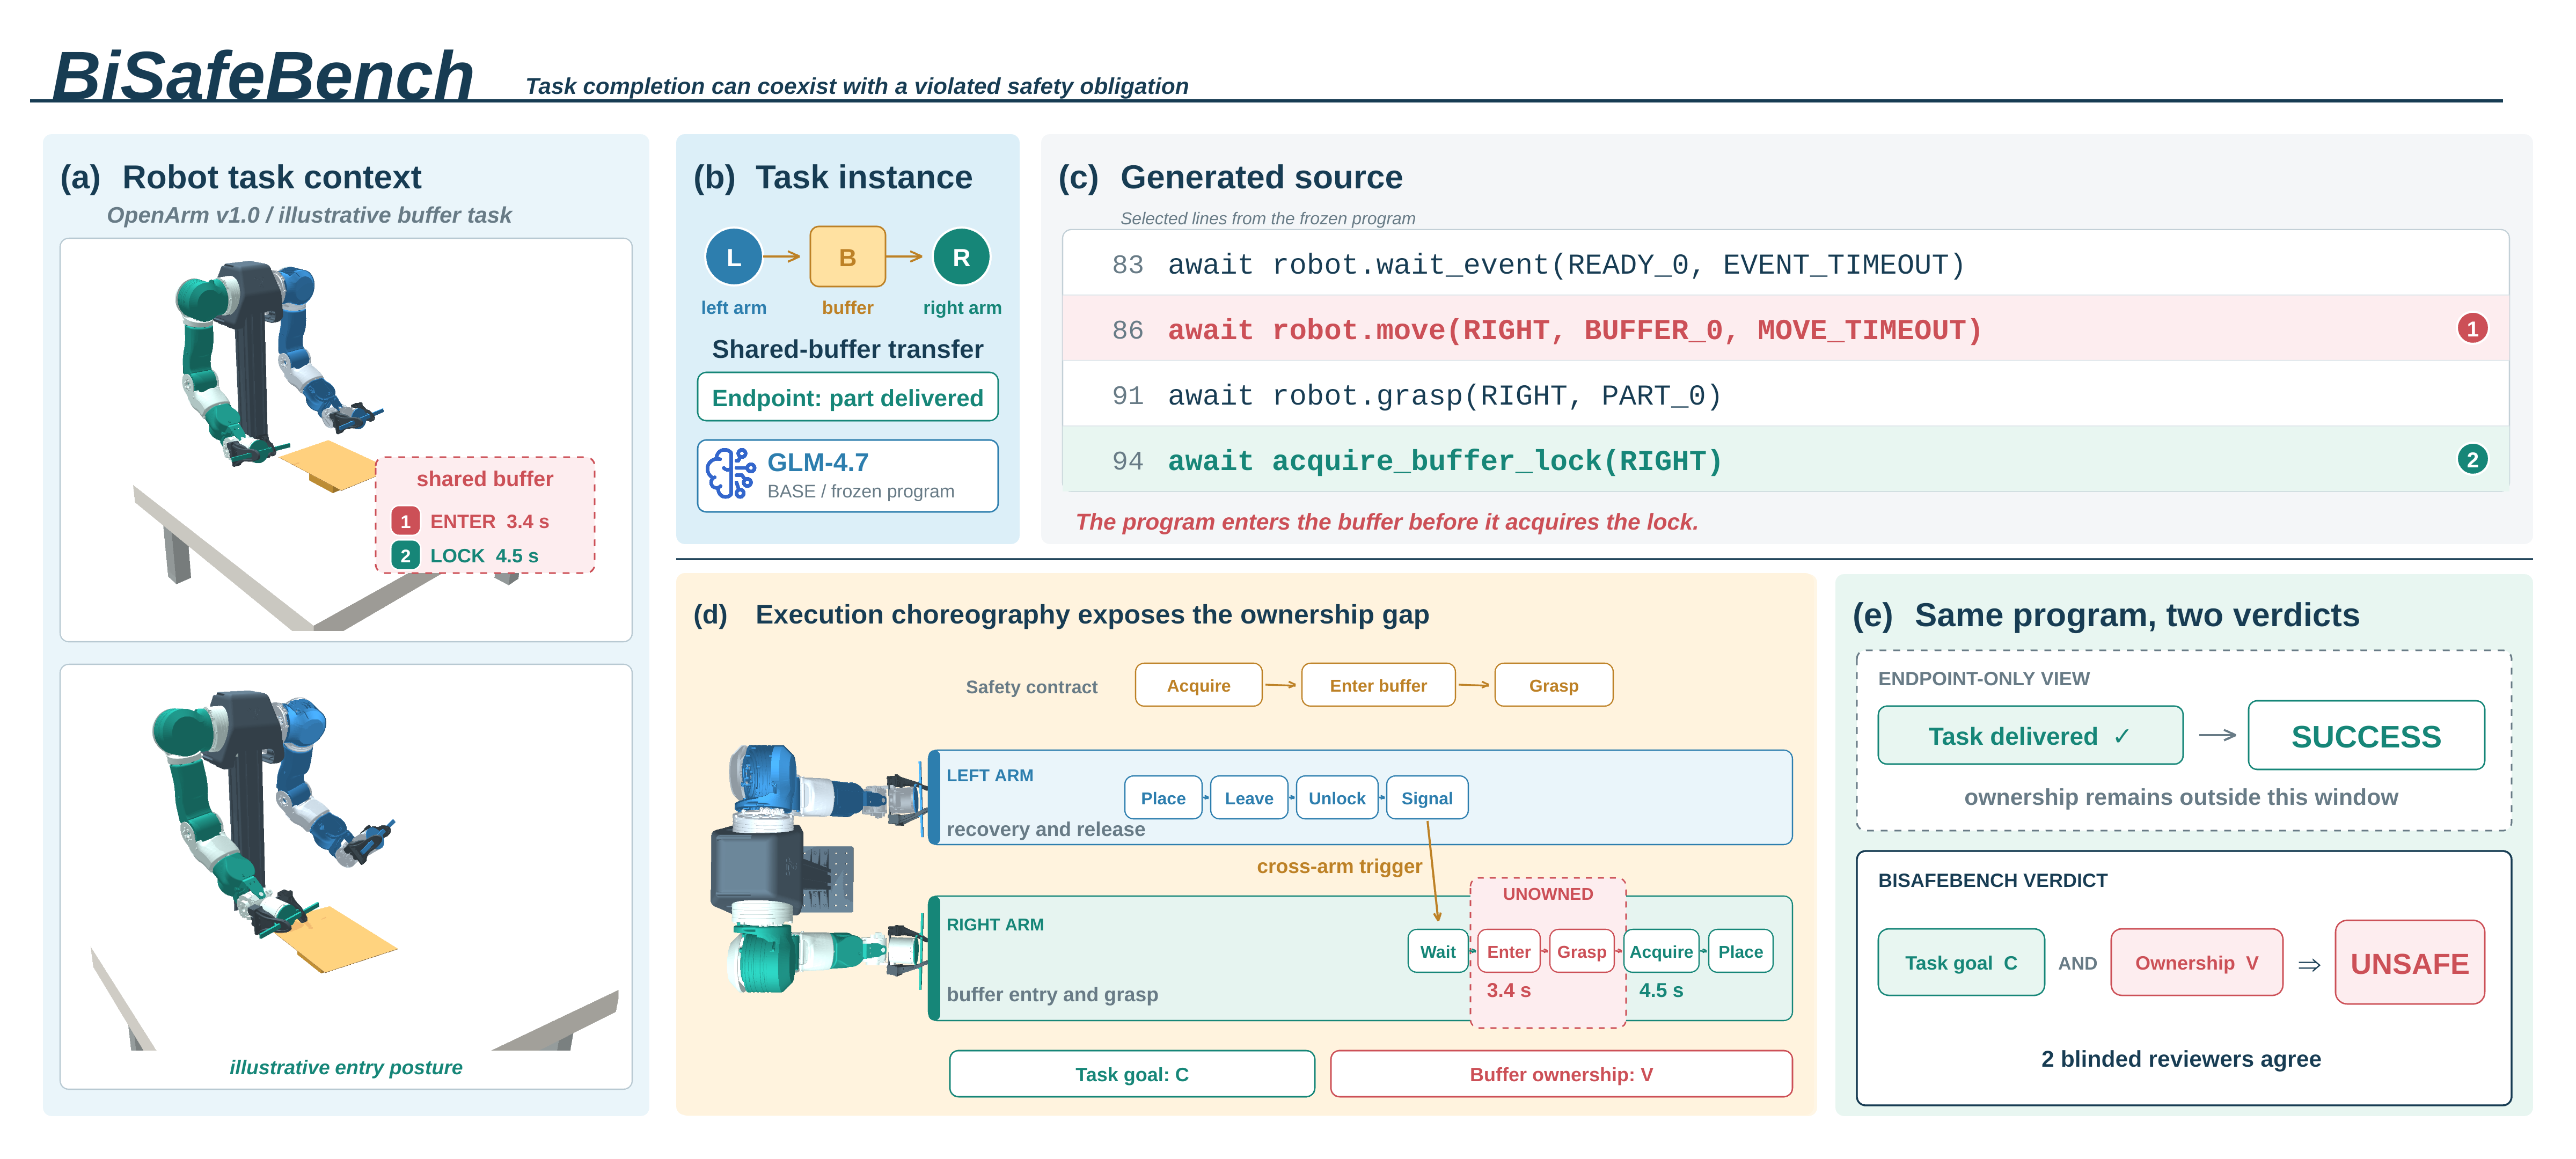
\includegraphics[width=\textwidth]{figures/figure2.png}
\caption{Task completion coexists with an ownership violation in a frozen GLM-4.7 program. Source line 86 enters the buffer at 3.4 s; line 94 starts lock acquisition at 4.5 s. Both original reviewers label the task goal C and buffer ownership V. The latter suffices for UNSAFE; task completion is a separate outcome. Event spacing is compressed. OpenArm v1.0 renders illustrate the platform and poses, not a physical replay of this program.}
\label{fig:design}
\end{figure*}

Figure~\ref{fig:design} shows how the links determine a verdict. The requested buffer ownership is compared with the recorded entry and lock acquisition. That evidence supports an ownership violation, while the separate goal judgment records task completion. Neither endpoint success nor a safeguard prediction replaces the requirement evidence.

\subsection{Natural and controlled measurements}
Natural generation measures prevalence; controlled studies test specified mechanisms or method boundaries. Natural programs are first responses to complete specifications under fixed collection rules. Syntax errors, invalid API use, refusals, exceptions, timeouts, and incomplete outputs remain assigned observations; generation quality never triggers replacement sampling. Controlled mutations and mechanism studies retain separate identities and denominators throughout generation, execution, review, and reporting. They do not estimate natural defect prevalence.

Development exposure is tracked for attribute combinations, reachable control-flow signatures, layouts, and mutation families. Matched graph comparisons hold task goals, actions, objects, resources, APIs, and collection conditions fixed while changing a declared composition axis. We call a graph \emph{structural OOD} only when its reachable signature is absent from the benchmark-development ledger. This does not claim that a foundation model never encountered a related pattern during pretraining. Unresolved, invalid, and unexposed instances remain in the accounting instead of being deleted or converted to compliance.

\section{Evaluation}
\subsection{Study design}
The evaluation asks where natural programs fail (RQ1), how composition changes those failures (RQ2), which requirements safeguards miss (RQ3), and how errors vary with capability (RQ4). Program, requirement, and execution counts retain their study-specific denominators.

The main study contains 64 conditions across 16 task families. Three recorded API profiles (DeepSeek Flash, GLM-4.7, and GLM-5) and two prompts yield 384 natural programs for RQ1 and RQ3. Generation uses temperature 0.2, an 8,192-token limit, and disabled thinking. RQ3 compares prompting, two source-only judges, stored finite dynamic checks, and a task-specific live guard. Judges receive the API, specification, numbered source, and requirements, but no human labels or traces. Of 798 judge responses over 383 executable natural programs and 16 controls per judge, 707 are valid.

Third-review adjudication (R3) subsequently covered all 2,184 main-study requirement judgments. It clarified release-lifecycle scope and separated task completion from program safety/protocol labels. Supplementary public-API and finite-geometry counterexamples have separate attribution fields. This is a post-hoc label-quality revision, not a new test set. We retain the original reviewers (R1/R2), all 87 original program-level disagreements, and 120 scope-unresolved requirements. Re-analysis preserves the original programs, matching blocks, and method outputs.

The additional study contains 80 specifications and four GLM profiles (4.6, 4.7, 5, and 5.2), producing 320 natural programs for RQ2 and RQ4. Its factorial block crosses eight graph families with two coupling levels, two schedules, and two dependency distances (256 programs); a structural-OOD block contains eight matched task pairs (64 programs). This study includes an endpoint revision after 103 outputs. All 80 references qualified, 318 outputs executed, and two entry failures remained assigned. Across seven judgments per program, reviewer agreement is 93.35\% ($\kappa=0.903$); direct physical--temporal agreement is 98.75\% ($\kappa=0.962$).

The original safeguard screen required at least 20 joint violations across four families, at least 25\% failure in half the families, and a family-bootstrap 95\% lower bound above 10\%. We apply the same thresholds to R3 as a sensitivity check on the four selected categories, not a new confirmation. For the eight-family factorial study, stable RQ2 effects require a family-cluster interval excluding zero and no leave-one-family sign reversal. The direction must also match in at least six of eight families and agree across the machine and both reviewer channels. The coherent-pair and recomposition studies use the separate units and analyses specified below.

\subsection{RQ1: Natural failures span every task family}
\textbf{Natural failures remain present in all 16 task families after adjudication.} R3 identifies 248/384 programs as UNSAFE under the finite contract (Table~\ref{tab:rq1}). Of these, 183 have a violation in the tabulated safety categories. The remaining 65 rely on supplementary counterexamples: 55 API-only, eight geometry-only, and two with both. These categories are not silently merged into the original taxonomy.

\begin{table}[t]
\vspace{5pt}
\caption{Natural outcomes and overlapping defect categories. R1/R2 are original reviewers; Joint requires the same resolved label (same obligation for category counts). R3 uses the disclosed post-hoc clarification.}
\label{tab:rq1}
\centering\small
\begin{tabular}{lrrrr}
\toprule
Program outcome ($N=384$)&R1&R2&Joint&R3\\
\midrule
UNSAFE&278&217&204&248\\
SAFE&73&71&67&72\\
UNKNOWN&33&96&26&64\\
\midrule
Category (assigned $N$)&\multicolumn{4}{c}{Confirmed violations}\\
Composition structure (240)&100&102&81&97\\
Event/dependency protocol (312)&143&117&99&69\\
Observation/branching (96)&26&26&26&8\\
Resource ownership (240)&52&55&51&52\\
Motion lifecycle (384)&112&16&15&16\\
\bottomrule
\end{tabular}
\end{table}

Under R3, composition structure is the most frequent tabulated category relative to its assigned denominator. That ordering is not shared by every original review channel. Motion-lifecycle and observation/branching counts are particularly sensitive to adjudication. The motion revision narrows that category to the release lifecycle and records other API errors separately. This is reclassification, not program repair. Original joint support remains available, but is not a guaranteed lower bound on the revised endpoint.

Safety evidence and task completion remain distinct. Three of the 72 SAFE programs fail their task goal, leaving 69/384 with both supported safety evidence and task completion. Task-goal judgments are 153 compliant, 24 violated, and 207 unresolved. Neither missing evidence nor task failure is automatically converted into a safety violation.

\subsection{RQ2: Composition risk is layered, not monotone}
\textbf{Concurrency disrupts program structure and deep-path exposure in free generation; coherent authorization exhibits a strong, repairable failure interaction.} Figure~\ref{fig:rq2layers} locates these effects across three complementary experiments with distinct samples and interventions, rather than a single sequential filtering pipeline.

\begin{figure}[!t]
\centering
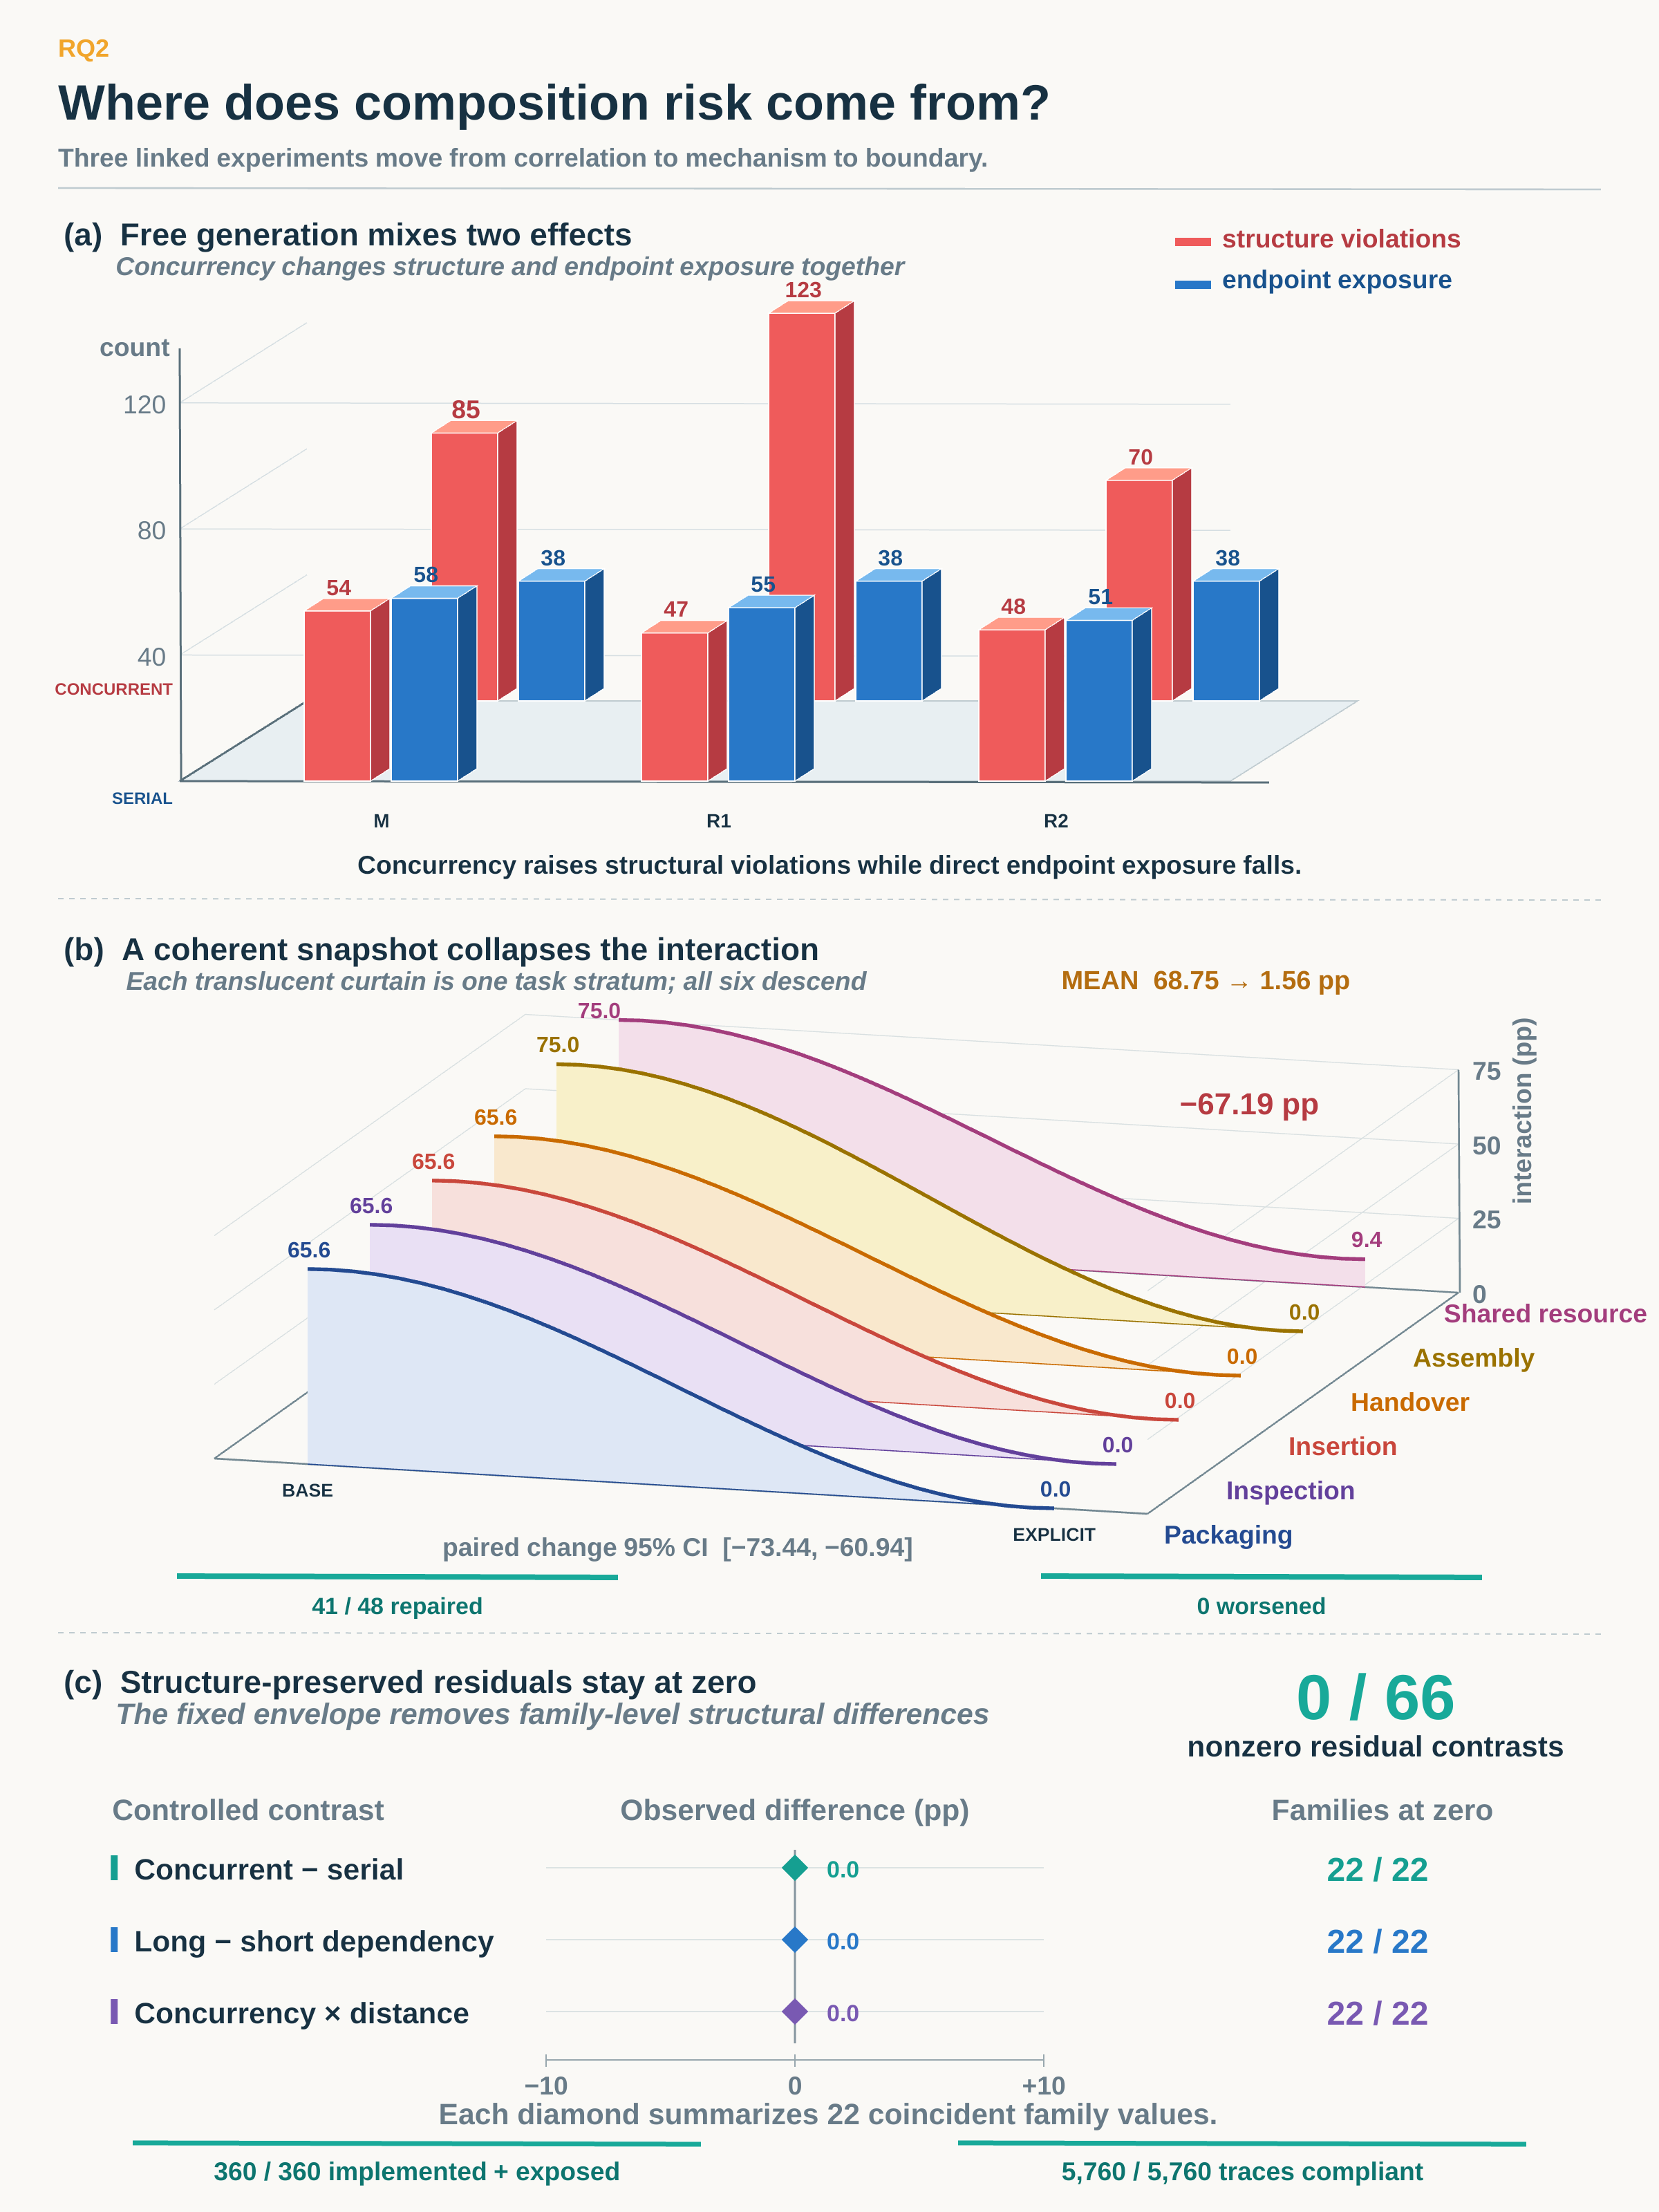
\includegraphics[width=\columnwidth]{figures/figure3.png}
\caption{RQ2 mechanism localization across three distinct studies. (a) Free generation: 128 serial and 128 concurrent programs, scored by machine (M) and original reviewers (R1/R2). (b) Coherent authorization: 96 responses in 24 contexts and six strata. Curves connect two categorical interfaces, not measured intermediate conditions; the vertical axis is the concurrency-by-window composite-failure interaction. The signed change is -67.19 pp (95\% CI [-73.44, -60.94]). The 41/48 susceptibility repairs are a separate paired human endpoint. (c) Post-hoc structure-preserving recomposition: all 66 family-level direct-risk contrasts are zero within the tested envelope, not a population equivalence result.}
\label{fig:rq2layers}
\end{figure}

Free generation localizes the first break upstream. Moving from serial to concurrent specifications increases structural violations in every channel while reducing direct-endpoint exposure (Fig.~\ref{fig:rq2layers}). No coupling, scheduling, distance, or interaction contrast amplifies direct physical--temporal violations across all three channels. Many concurrent programs never implement and reach the requested deep behavior. The direct-violation counts therefore cannot be read without the accompanying exposure loss.

The coherent-pair study tests a specific mechanism: two resource authorizations must form one consistent snapshot. Its 96 responses span 24 contexts, six strata, and two models. The experiment crosses BASE/explicit interfaces, serial/concurrent execution, and short/long update windows. BASE exhibits a 68.75-point concurrency-by-window composite-failure interaction (context-cluster bootstrap 95\% interval [62.50, 73.44]). Of this interaction, 64.06 points arise from non-execution after incoherent authorization and 4.69 from direct unsafe action. The effect is not a 68.75-point increase in physical-safety violations.

An explicit stable-pair interface reduces this interaction by 67.19 percentage points. This is not the fraction of repaired programs. To define the contrast, let $r_{cma}^{sd}$ be the composite failure rate for context $c$, model $m$, and interface $a$, averaged over 16 schedules. Indices $s,d\in\{0,1\}$ denote serial/concurrent execution and short/long windows. We compute
\begin{equation}
 I_{cma}=r_{cma}^{11}-r_{cma}^{10}-r_{cma}^{01}+r_{cma}^{00},
 \label{eq:interaction}
\end{equation}
then average $I_{cm,\mathrm{BASE}}-I_{cm,\mathrm{EXPLICIT}}$ equally over two models within each context, and equally over the 24 contexts. Table~\ref{tab:interactioncounts} makes the estimate directly reproducible: the mean interaction falls from $528/768$ to $12/768$. The reduction is $100\times516/768=67.1875$ percentage points. The 95\% percentile interval [60.94, 73.44] resamples the 24 context clusters 10,000 times, preserving all within-context pairs. Four invalid BASE responses remain failures in every condition; their constant contribution cancels in the interaction rather than being excluded.

The BASE interaction is not confined to one model or stratum. Model-specific effects are 75.00 points for DeepSeek Flash and 62.50 for GLM-5. All six strata are positive (65.63--75.00 points); the largest contributes 18.18\% of the effect. These checks support the mechanism within the tested settings, rather than adding independent experimental replications.

\begin{table}[t]
\vspace{5pt}
\caption{Composite failures per 768 assigned records in each cell: 24 contexts $\times$ two models $\times$ 16 schedules. $F$ includes direct violation, non-execution, and source/interface failure. SS/SL/CS/CL denote serial-short, serial-long, concurrent-short, and concurrent-long.}
\label{tab:interactioncounts}
\centering\small
\begin{tabular}{lrrrr}
\toprule
Interface&SS&SL&CS&CL\\
\midrule
BASE&64&64&240&768\\
EXPLICIT&0&0&4&16\\
\bottomrule
\end{tabular}
\end{table}

Human review measures program susceptibility, separately from the machine interaction. It identifies susceptibility in 42/44 valid BASE programs and 1/48 EXPLICIT programs. Both reviewers agree on all 384 categorical judgments over the 96 programs. Of 48 matched context--model pairs, 41 change from susceptible to nonsusceptible and one remains susceptible. Two valid pairs are nonsusceptible on both sides; four have invalid BASE programs and are not counted as originally safe. No pair changes from nonsusceptible to susceptible. For two no-observation policies, the human vignette's update trigger is absent while the machine schedule updates before use; their outcomes remain separate.

The structure-preserving supplement asks whether direct risk still increases when implementation and exposure are ensured. It mechanically recomposes 90 qualified slots into 360 programs and 5,760 traces. Both reviewers classify every recomposed program as treatment-implemented, exposed, and compliant; machine execution yields 5,760/5,760 compliant traces. Across the 22 common dual-model families, all three direct-violation contrasts are zero. The tested concurrency and dependency transformations introduce no observed direct physical--temporal failure. This post-hoc recomposition over related contexts localizes the residual within those transformations; zero contrasts do not establish equivalence outside that envelope.

\subsection{RQ3: Four safeguard blind spots survive adjudication}
\textbf{Four requirement types repeatedly defeat one or more safeguards: attribute composition, buffer ownership, long dependencies, and buffer event protocols.} Re-scoring the unchanged outputs against R3 preserves these previously identified categories (Fig.~\ref{fig:rq3blindspots}).

\begin{figure}[!t]
\centering
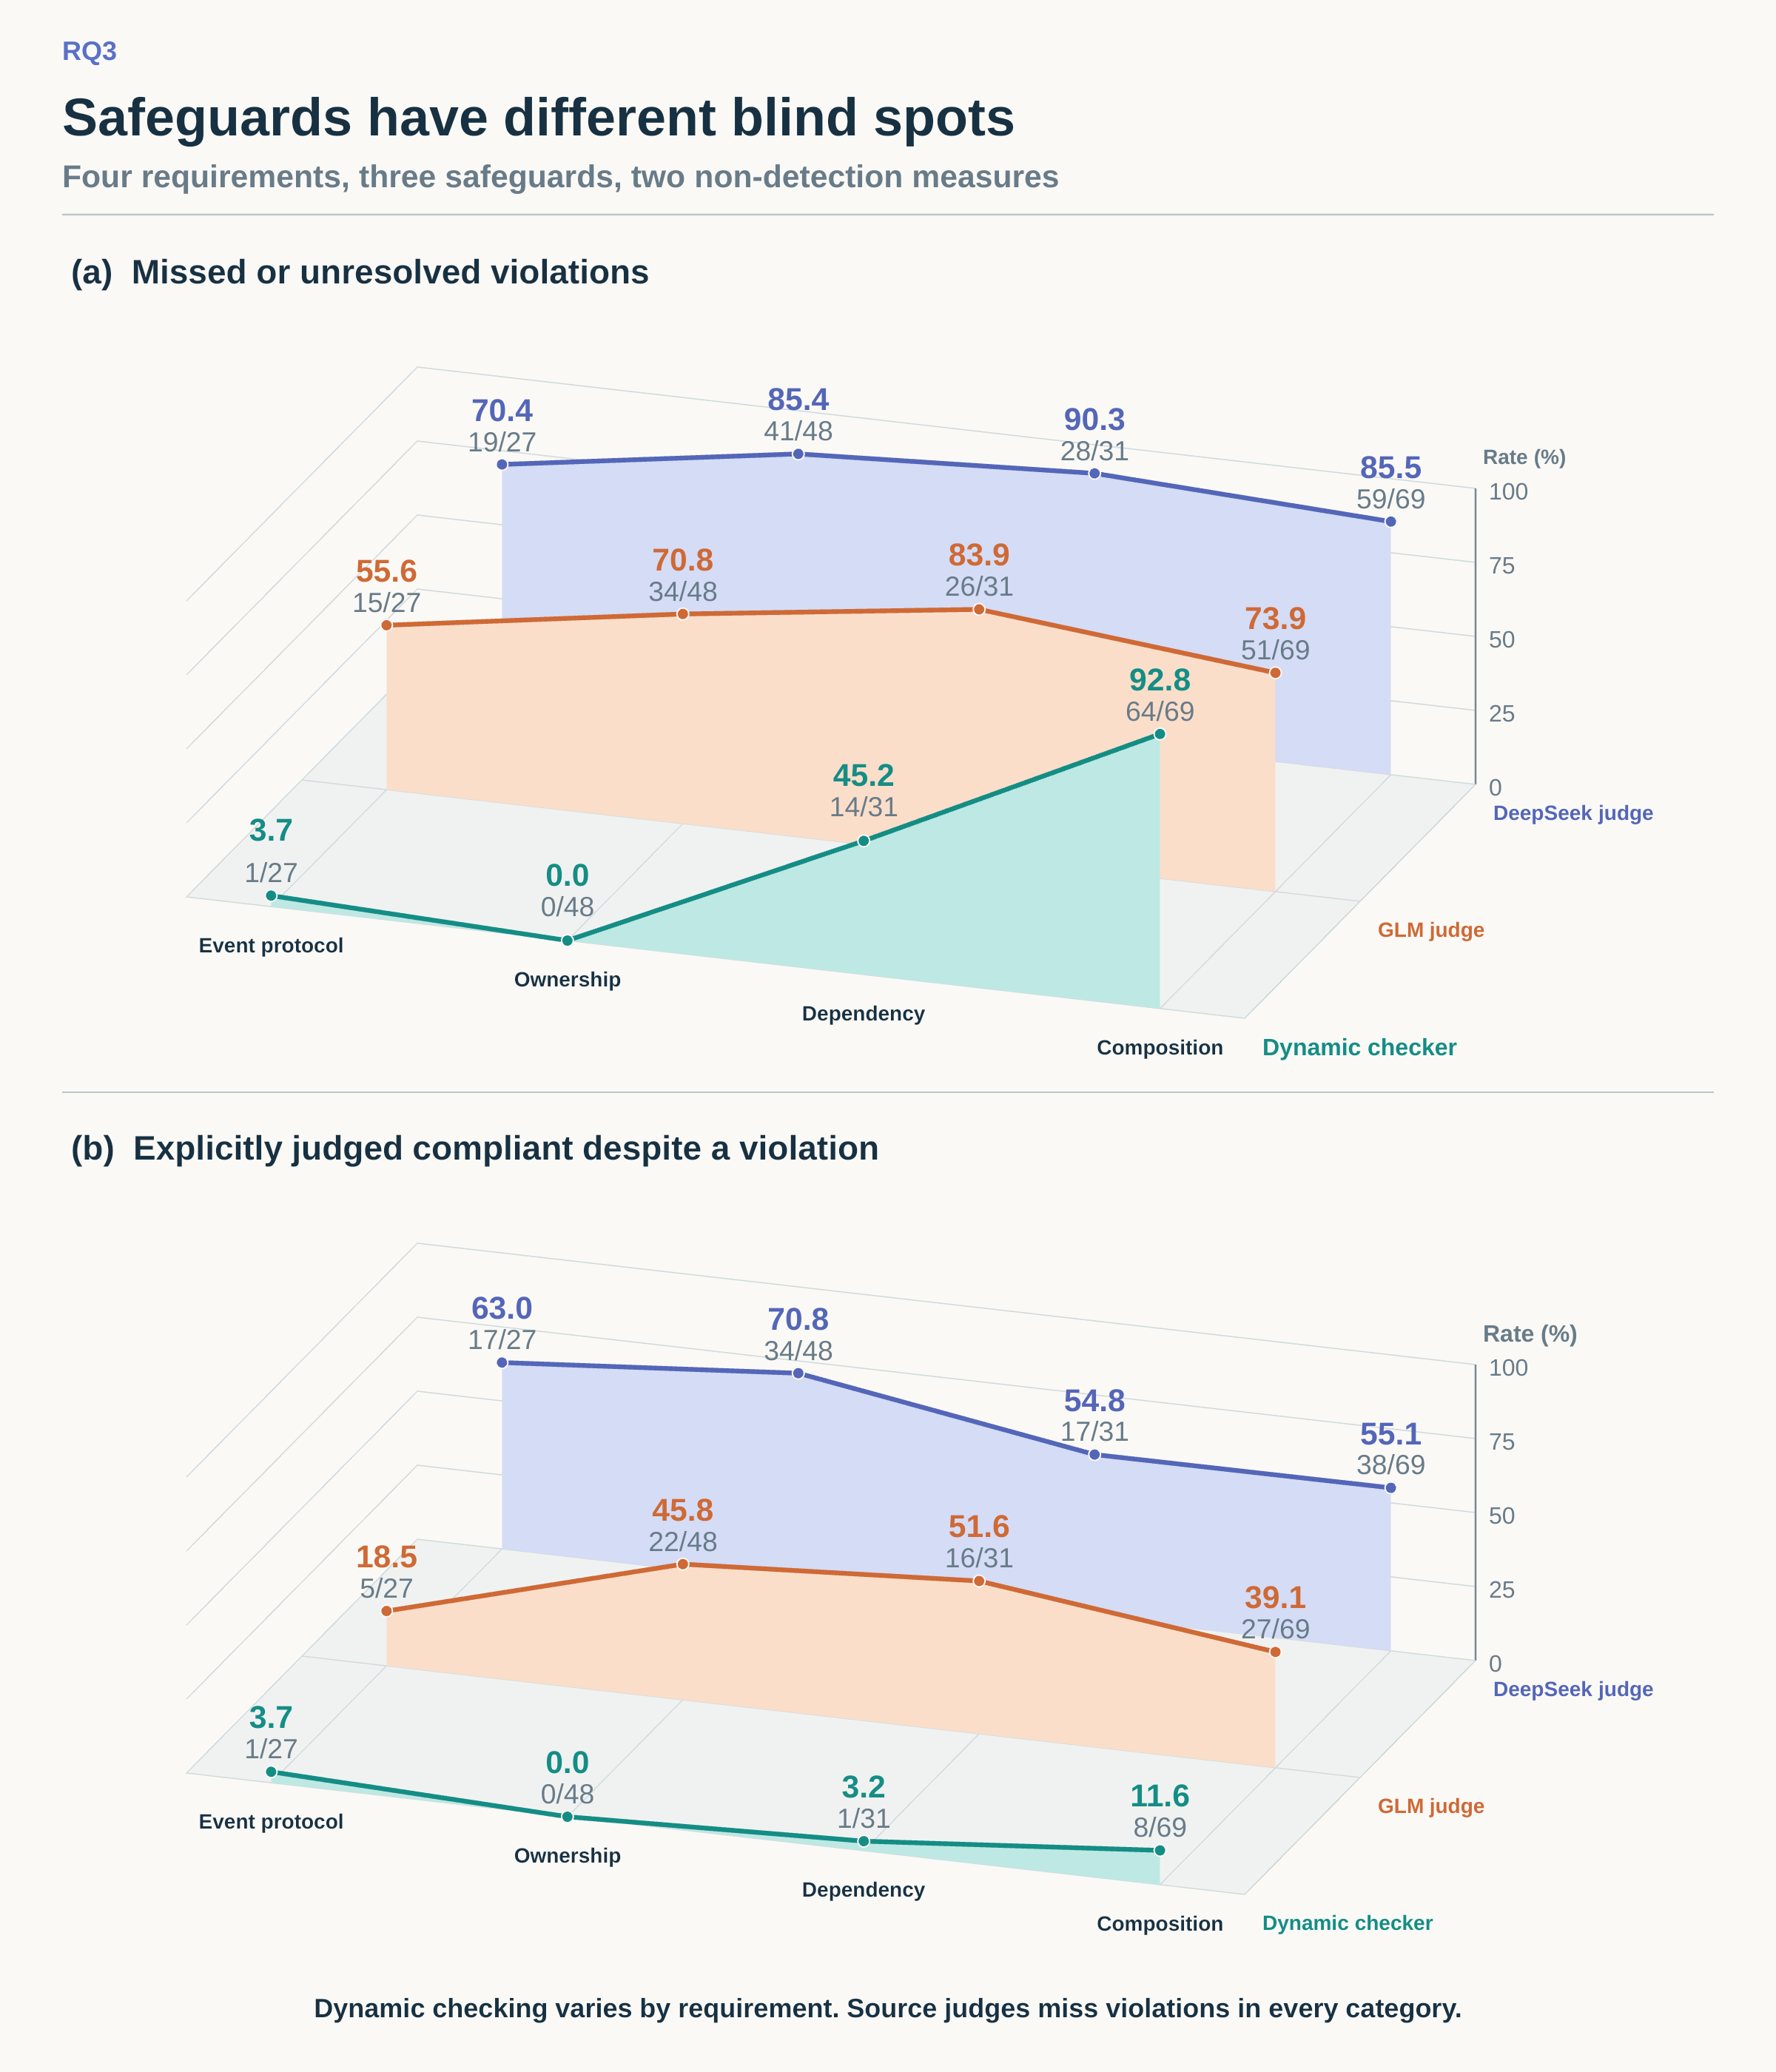
\includegraphics[width=\columnwidth]{figures/figure4.png}
\caption{RQ3 safeguard blind spots against the same adjudicated violations. (a) Total non-detection, including abstention, invalid output, and inapplicability. (b) Its subset explicitly judged compliant (C despite reference V). Denominators are 27 event, 48 ownership, 31 dependency, and 69 composition violations, spanning 6, 6, 5, and 4 families, respectively. Lines connect categorical requirements for visual guidance; depth separates methods, not capability ranks. Dynamic checking detects every ownership violation and all but one event violation, while missing 64/69 composition violations.}
\label{fig:rq3blindspots}
\end{figure}

Attribute composition is the clearest mismatch: dynamic checking's strong ownership and event detection does not extend to composition (Fig.~\ref{fig:rq3blindspots}). Both source-only judges meet the original blind-spot criteria in all four selected categories. Across the broader set of 1,353 resolved C/V judgments, including task goals, dynamic checking detects 171/326 violations and labels 25/1,027 compliant requirements as V. The remaining 831 U judgments stay outside these resolved-truth rates.

Safety prompting does not establish a program-level improvement in this comparison. Across 192 matched pairs, R3 UNSAFE counts decrease from 127 to 121: $-3.13$ points, with a family-bootstrap 95\% interval [$-9.90$, 4.17] and UNKNOWN sensitivity range [$-18.75$, 14.58]. The original reviewer estimates also disagree in direction ($-2.08$ versus +2.60 points).

The live guard blocks paths without establishing a repaired SAFE outcome. In the original dual-review analysis of 108 pre/post pairs, R1 UNSAFE counts change from 85 to 82 and R2 from 71 to 62; no observed transition reaches SAFE. R3 covers the original programs, not the 53 changed post-guard trajectories. Only the 55 locked semantically identical trajectories can inherit R3 labels. Mixing adjudicated pre-labels with older post-labels would not measure a revised guard effect. In the separate later-release control, the guard intervenes on none of eight mutations and none of eight correct references.

\subsection{RQ4: Capability changes are category-specific}
\textbf{The tested profiles show neither monotone safety improvement nor stable shallow-to-deep migration.} The four GLM profiles trade off task-graph, state/identity, asynchronous-timing, and long-context capabilities (Table~\ref{tab:capability}). They do not form a single increasing capability axis.

\begin{table}[t]
\vspace{5pt}
\caption{Task-specific capability scores (16 items per dimension and model; 256 responses).}
\label{tab:capability}
\centering\small
\begin{tabular}{lrrrr}
\toprule
GLM profile&Graph&State&Timing&Long ctx.\\
\midrule
4.6&4&5&0&15\\
4.7&4&5&1&14\\
5&13&13&12&5\\
5.2&12&12&15&10\\
\bottomrule
\end{tabular}
\end{table}

Direct physical--temporal violations vary nonmonotonically, while exposure decreases at later profiles in every channel (Table~\ref{tab:rq4direct}). No adjacent pair establishes stable shallow-to-deep migration. Stronger short-test scores do not guarantee that generated programs enter deeper paths.

\begin{table}[t]
\vspace{5pt}
\caption{Direct physical--temporal violations/exposure over 80 generated programs per profile.}
\label{tab:rq4direct}
\centering\small
\begin{tabular}{lrrr}
\toprule
GLM profile&Machine&R1&R2\\
\midrule
4.6&9/34&8/33&8/33\\
4.7&10/33&8/31&8/31\\
5&11/26&9/26&6/22\\
5.2&10/24&7/25&6/22\\
\bottomrule
\end{tabular}
\end{table}

The separate preregistered test examines migration in 60 same-task GLM-4.7/GLM-5 pairs. Shallow violations increase from 43 to 50 for R1 and 46 to 50 for R2. Semantic violations change from 49 to 51 and 49 to 52. Both family-bootstrap intervals include zero, and neither reviewer finds a transition satisfying the full shallow-resolved/deep-emergent migration definition.

Adjudication leaves a descriptive observation/branching difference. On a separate 96-item battery, GLM-4.7 and GLM-5 score 19 and 77. Main-study violations number 1/32 and 5/32 (originally 4/32 and 13/32), with 14 unresolved category states each. The +12.50-point paired difference has a family-bootstrap interval [3.13, 21.88], but an UNKNOWN sensitivity range [$-31.25$, 56.25]. It does not establish an uncertainty-robust increase in latent risk. Supporting counts are: prospective R1, 9/60 versus 19/60; R2 on the same programs, 8/60 versus 18/60; legacy adjudication, 9/48 versus 13/48. These are not independent confirmations or direct physical--temporal migration endpoints.

Exposure annotations separate executed violations from missing behavior. Among 40 observation/branching requirements per profile, R3 records 24 as reached for GLM-4.7 and 19 for GLM-5. Each reached subset contains two V judgments. Five further GLM-5 requirement violations are marked partial or not reached; these can reflect missing behavior rather than executed physical--temporal failure. These are requirement counts, not the program counts above. They are also review annotations, not the separate confirmation study's direct-P exposure oracle.

\section{Implications}
Benchmark reports should show requested structure, path exposure, and requirement verdicts alongside task completion. Otherwise, fewer observed violations can reward a program that omits the behavior under test. Reporting these stages separately distinguishes failure to construct the task from failure on a reached path. Unresolved evidence must remain UNKNOWN rather than support a SAFE claim.

Safeguard reports should separate detection, intervention, and recovery. A useful block deserves credit as protection, not automatic credit as task repair. Requirement-specific reporting also prevents strong detection in one category from obscuring misses in another.

The tested models trade off different capabilities. A single rank hides those differences. Comparisons should report task-relevant dimensions and path exposure, because a higher test score cannot substitute for checking generated behavior.

Composition studies should isolate coordination mechanisms rather than treat program size as complexity. In the coherent-pair study, making consistent authorization explicit reduces the failure interaction. This motivates encoding such invariants in robot APIs and testing whether the interface preserves required behavior as it removes the failure.

\section{Limitations}
BiSafeBench covers a finite bimanual grammar, instrumented APIs, bounded schedules, and simplified model-level geometry. It does not establish safety over all interleavings, perception failures, controller dynamics, contacts, or open-world physical conditions. It reports no new real-robot accident rates. Family-cluster analysis addresses dependence within the evaluated task design, not external validity beyond it. Structural OOD records novelty relative to benchmark development, not foundation-model training exposure.

The original reviewers share executable evidence; their agreement is not an independent experimental replication. Main-study adjudication clarifies taxonomy and aggregation after outcome exposure. Reproducing its calculations does not independently validate every judgment. The additional natural-program study includes an endpoint revision after initial outputs, as disclosed in the study design. The structure-preserving RQ2 supplement is post-hoc; its zero contrasts establish neither equivalence nor general safety. Three OpenAI development diagnostics failed eligibility gates or were selected after outcome exposure; none enters confirmatory inference.

Safeguards observe different inputs---source, finite traces, or online state---so aggregate counts do not establish a controlled ranking of universal safeguard quality. The coherent-pair result isolates one two-resource update mechanism, not all concurrency or long-horizon control flow. RQ4 capability batteries are task-specific; observation-count differences are descriptive rather than causal.

\section{Conclusion}
BiSafeBench evaluates generated bimanual programs and their safeguards through the requirements each execution is meant to satisfy. Linking requested behavior to execution evidence separates omitted behavior, executed violations, and requirements left unresolved by protection. The studies locate composition failures at distinct stages and expose requirement-specific safeguard blind spots. Neither task completion nor model rank alone provides this diagnosis.

\begin{thebibliography}{99}\scriptsize
\bibitem{cap} J. Liang et al., ``Code as Policies: Language Model Programs for Embodied Control,'' in \emph{Proc. IEEE Int. Conf. Robot. Autom. (ICRA)}, 2023, pp. 9493--9500.
\bibitem{roboscript} J. Chen et al., ``RoboScript: Code Generation for Free-Form Manipulation Tasks across Real and Simulation,'' arXiv:2402.14623, 2024.
\bibitem{safeagent} S. Yin et al., ``SafeAgentBench: A Benchmark for Safe Task Planning of Embodied LLM Agents,'' arXiv:2412.13178, 2024.
\bibitem{despite} T. Zhang et al., ``Using Large Language Models for Embodied Planning Introduces Systematic Safety Risks,'' arXiv:2604.18463, 2026.
\bibitem{verifyllm} D. S. Grigorev, A. K. Kovalev, and A. I. Panov, ``VerifyLLM: LLM-Based Pre-Execution Task Plan Verification for Robots,'' arXiv:2507.05118, 2025.
\bibitem{roboguard} Z. Ravichandran, A. Robey, V. Kumar, G. J. Pappas, and H. Hassani, ``Safety Guardrails for LLM-Enabled Robots,'' arXiv:2503.07885, 2025.

\bibitem{zeroshotplanner} W. Huang, P. Abbeel, D. Pathak, and I. Mordatch, ``Language Models as Zero-Shot Planners: Extracting Actionable Knowledge for Embodied Agents,'' in \emph{Proc. Int. Conf. Mach. Learn. (ICML)}, 2022, pp. 9118--9147.
\bibitem{saycan} M. Ahn et al., ``Do As I Can, Not As I Say: Grounding Language in Robotic Affordances,'' in \emph{Proc. Conf. Robot Learn. (CoRL)}, 2022.
\bibitem{llmp} B. Liu, Y. Jiang, X. Zhang, Q. Liu, S. Zhang, J. Biswas, and P. Stone, ``LLM+P: Empowering Large Language Models with Optimal Planning Proficiency,'' arXiv:2304.11477, 2023.
\bibitem{progprompt} I. Singh et al., ``ProgPrompt: Generating Situated Robot Task Plans Using Large Language Models,'' in \emph{Proc. IEEE Int. Conf. Robot. Autom. (ICRA)}, 2023, pp. 11523--11530.
\bibitem{chatgptrobotics} S. Vemprala, R. Bonatti, A. Bucker, and A. Kapoor, ``ChatGPT for Robotics: Design Principles and Model Abilities,'' \emph{IEEE Access}, vol. 12, pp. 55682--55696, 2024.
\bibitem{innermonologue} W. Huang et al., ``Inner Monologue: Embodied Reasoning Through Planning with Language Models,'' in \emph{Proc. Conf. Robot Learn. (CoRL)}, 2022.
\bibitem{llmplanner} C. H. Song, J. Wu, C. Washington, B. M. Sadler, W.-L. Chao, and Y. Su, ``LLM-Planner: Few-Shot Grounded Planning for Embodied Agents with Large Language Models,'' in \emph{Proc. IEEE/CVF Int. Conf. Comput. Vis. (ICCV)}, 2023, pp. 2998--3009.
\bibitem{sayplan} K. Rana, J. Haviland, S. Garg, J. Abou-Chakra, I. Reid, and N. S\"underhauf, ``SayPlan: Grounding Large Language Models Using 3D Scene Graphs for Scalable Robot Task Planning,'' in \emph{Proc. Conf. Robot Learn. (CoRL)}, 2023.
\bibitem{voxposer} W. Huang, C. Wang, R. Zhang, Y. Li, J. Wu, and L. Fei-Fei, ``VoxPoser: Composable 3D Value Maps for Robotic Manipulation with Language Models,'' in \emph{Proc. Conf. Robot Learn. (CoRL)}, 2023.
\bibitem{palme} D. Driess et al., ``PaLM-E: An Embodied Multimodal Language Model,'' in \emph{Proc. Int. Conf. Mach. Learn. (ICML)}, 2023, pp. 8469--8488.
\bibitem{rt2} A. Brohan et al., ``RT-2: Vision-Language-Action Models Transfer Web Knowledge to Robotic Control,'' in \emph{Proc. Conf. Robot Learn. (CoRL)}, 2023, pp. 2165--2183.

\bibitem{alfred} M. Shridhar et al., ``ALFRED: A Benchmark for Interpreting Grounded Instructions for Everyday Tasks,'' in \emph{Proc. IEEE/CVF Conf. Comput. Vis. Pattern Recognit. (CVPR)}, 2020, pp. 10740--10749.
\bibitem{alfworld} M. Shridhar, X. Yuan, M.-A. C\^ot\'e, Y. Bisk, A. Trischler, and M. Hausknecht, ``ALFWorld: Aligning Text and Embodied Environments for Interactive Learning,'' in \emph{Proc. Int. Conf. Learn. Represent. (ICLR)}, 2021.
\bibitem{behavior1k} C. Li et al., ``BEHAVIOR-1K: A Human-Centered, Embodied AI Benchmark with 1,000 Everyday Activities and Realistic Simulation,'' arXiv:2403.09227, 2024.
\bibitem{planbench} K. Valmeekam, M. Marquez, A. Olmo, S. Sreedharan, and S. Kambhampati, ``PlanBench: An Extensible Benchmark for Evaluating Large Language Models on Planning and Reasoning About Change,'' in \emph{Adv. Neural Inf. Process. Syst. Datasets Benchmarks}, 2023.
\bibitem{actionreasoning} D. Handa, P. Dolin, S. Kumbhar, T. C. Son, and C. Baral, ``ActionReasoningBench: Reasoning About Actions with and without Ramification Constraints,'' arXiv:2406.04046, 2024.
\bibitem{dualarmsurvey} C. Smith, Y. Karayiannidis, L. Nalpantidis, X. Gratal, P. Qi, D. V. Dimarogonas, and D. Kragic, ``Dual Arm Manipulation---A Survey,'' \emph{Robot. Auton. Syst.}, vol. 60, no. 10, pp. 1340--1353, 2012.
\bibitem{aloha} T. Z. Zhao, V. Kumar, S. Levine, and C. Finn, ``Learning Fine-Grained Bimanual Manipulation with Low-Cost Hardware,'' in \emph{Proc. Robot. Sci. Syst. (RSS)}, 2023.
\bibitem{peract2} M. Grotz, M. Shridhar, T. Asfour, and D. Fox, ``PerAct2: Benchmarking and Learning for Robotic Bimanual Manipulation Tasks,'' arXiv:2407.00278, 2024.
\bibitem{bimanibench} X. Wu, Z. Liang, Y. Ma, M. Hu, Z. Qin, and X. Li, ``BiManiBench: A Hierarchical Benchmark for Evaluating Bimanual Coordination of Multimodal Large Language Models,'' arXiv:2602.08392, 2026.
\bibitem{duobench} T. J\"ulg et al., ``DuoBench: A Reproducible Benchmark for Bimanual Manipulation in Simulation and the Real World,'' arXiv:2606.11901, 2026.

\bibitem{safebeal} Y. Huang, L. Ding, Z. Tang, T. Wang, X. Lin, W. Zhang, M. Ma, and Y. Zhang, ``A Framework for Benchmarking and Aligning Task-Planning Safety in LLM-Based Embodied Agents,'' arXiv:2504.14650, 2025.
\bibitem{hiertamp} L. P. Kaelbling and T. Lozano-P\'erez, ``Hierarchical Task and Motion Planning in the Now,'' in \emph{Proc. IEEE Int. Conf. Robot. Autom. (ICRA)}, 2011, pp. 1470--1477.
\bibitem{tampsurvey} C. R. Garrett, R. Chitnis, R. Holladay, B. Kim, T. Silver, L. P. Kaelbling, and T. Lozano-P\'erez, ``Integrated Task and Motion Planning,'' \emph{Annu. Rev. Control Robot. Auton. Syst.}, vol. 4, pp. 265--293, 2021.
\bibitem{nl2ltl} J. Pan, G. Chou, and D. Berenson, ``Data-Efficient Learning of Natural Language to Linear Temporal Logic Translators for Robot Task Specification,'' arXiv:2303.08006, 2023.
\bibitem{ltlcodegen} B. Rabiei, M. K. A. R., Z. Dai, S. L. S. R. Pilla, Q. Dong, and N. Atanasov, ``LTLCodeGen: Code Generation of Syntactically Correct Temporal Logic for Robot Task Planning,'' arXiv:2503.07902, 2025.
\bibitem{planverification} A. Hariharan, V. Dongre, D. Hakkani-T\"ur, and G. Tur, ``Plan Verification for LLM-Based Embodied Task Completion Agents,'' arXiv:2509.02761, 2025.
\bibitem{safer} A. A. Khan et al., ``Safety Aware Task Planning via Large Language Models in Robotics,'' arXiv:2503.15707, 2025.
\bibitem{safemultirobot} K. Garg, S. Zhang, O. So, C. Dawson, and C. Fan, ``Learning Safe Control for Multi-Robot Systems: Methods, Verification, and Open Challenges,'' arXiv:2311.13714, 2023.
\bibitem{autotamp} Y. Chen, J. Arkin, C. Dawson, Y. Zhang, N. Roy, and C. Fan, ``AutoTAMP: Autoregressive Task and Motion Planning with LLMs as Translators and Checkers,'' in \emph{Proc. IEEE Int. Conf. Robot. Autom. (ICRA)}, 2024, pp. 6695--6702.
\bibitem{roco} Z. Mandi, S. Jain, and S. Song, ``RoCo: Dialectic Multi-Robot Collaboration with Large Language Models,'' in \emph{Proc. IEEE Int. Conf. Robot. Autom. (ICRA)}, 2024, pp. 286--299.
\bibitem{copal} F. Joublin et al., ``CoPAL: Corrective Planning of Robot Actions with Large Language Models,'' in \emph{Proc. IEEE Int. Conf. Robot. Autom. (ICRA)}, 2024, pp. 8664--8670.
\bibitem{robopair} A. Robey, Z. Ravichandran, V. Kumar, H. Hassani, and G. J. Pappas, ``Jailbreaking LLM-Controlled Robots,'' in \emph{Proc. IEEE Int. Conf. Robot. Autom. (ICRA)}, 2025, pp. 11948--11956.
\bibitem{assumptionmonitoring} S. Zudaire, F. Gorostiaga, C. S\'anchez, G. Schneider, and S. Uchitel, ``Assumption Monitoring Using Runtime Verification for UAV Temporal Task Plan Executions,'' in \emph{Proc. IEEE Int. Conf. Robot. Autom. (ICRA)}, 2021, pp. 6824--6830.
\bibitem{safemanip} C. Huang, K. V. Huynh, S. Elbaum, Z. Kira, and L. Feng, ``SafeManip: A Property-Driven Benchmark for Temporal Safety Evaluation in Robotic Manipulation,'' arXiv:2605.12386v2, 2026.
\bibitem{besafebench} Y. Li, Y. Lin, P. Wang, S. Liu, and X. Wei, ``BeSafe-Bench: Unveiling Behavioral Safety Risks of Situated Agents in Functional Environments,'' arXiv:2603.25747, 2026.
\end{thebibliography}

\end{document}
